\documentclass{bioinfo}
\usepackage{hyperref}
\usepackage{subcaption}
\copyrightyear{2017} \pubyear{2017}

\access{Advance Access Publication Date: Day Month Year}
\appnotes{Manuscript Category}

\begin{document}
\firstpage{1}

\subtitle{Systems Biology}

\title[DFBA Models in SBML]{Dynamic Flux Balance Analysis Models in SBML}
\author[Watanabe \textit{et~al}.]{Leandro H. Watanabe\,$^{\text{\sfb 1}, \dagger}$\, Matthias K{\"o}nig\,$^{\text{\sfb 2}, \dagger}$\, and Chris J. Myers\,$^{\text{\sfb 1,}*}$}
\address{$^{\text{\sf 1}}$Department of Electrical and Computer Engineering, University of Utah, Salt Lake City, 84112, USA \\ 
$^{\text{\sf 2}}$Humboldt-University Berlin, Institute for Theoretical Biology, Institute for Biology,
Invalidenstra{\ss}e 43, 10115 Berlin, Germany}

\corresp{$^\ast$To whom correspondence should be addressed.\\ $^\dagger$Equal contribution.}

\history{}

\editor{}

%%%%%%%%%%%%%%%%%%%%%%%%%%%%%%%%%%%%%%%%%%%%
% ABSTRACT
%%%%%%%%%%%%%%%%%%%%%%%%%%%%%%%%%%%%%%%%%%%%
\abstract{\textbf{Motivation:} Systems biology models are typically simulated using a single formalism such as ordinary differential equations (ODE) or stochastic methods. However, more complex models require the coupling of multiple formalisms since different biological concepts are better described using different methods, e.g., stationary metabolism is often modeled using flux-balance analysis (FBA) whereas dynamic changes of model components are better described via ODEs. The coupling of FBA and ODE frameworks results in dynamic FBA models. A major challenge is how to describe such hybrid models coupling multiple frameworks in a standardized way, so that they can be exchanged between tools and simulated consistently and in a reproducible manner.\\
\textbf{Results:} This paper presents a scheme and implementation for encoding dynamic FBA models in the Systems Biology Markup Language (SBML), thereby allowing to exchange multi-framework computational models between software tools. The paper shows the feasibility of the approach using various example models and demonstrates that different tools are able to simulate the hybrid models and agree on the results. As part of this work, two independent implementations of a multi-framework simulation method for dynamic FBA have been developed supporting such models: \texttt{iBioSim} and \texttt{sbmlutils}.\\
\textbf{Availability:} All materials and models are available from \href{https://github.com/matthiaskoenig/dfba}{https://github.com/matthiaskoenig/dfba}. The tools used in this project are freely available: \texttt{iBioSim} at \href{http://www.async.ece.utah.edu/ibiosim}{http://www.async.ece.utah.edu/ibiosim} and \texttt{sbmlutils} at \href{https://github.com/matthiaskoenig/sbmlutils/}{https://github.com/matthiaskoenig/sbmlutils/}.\\
\textbf{Contact:} \href{myers@ece.utah.edu}{myers@ece.utah.edu}\\}
\maketitle

% DFBA: dynamic flux balance analysis
% FBA: flux balance analysis
% ODE: ordinary differential equations
% SOA: static optimization approach

%%%%%%%%%%%%%%%%%%%%%%%%%%%%%%%%%%%%%%%%%%%%
% INTRODUCTION
%%%%%%%%%%%%%%%%%%%%%%%%%%%%%%%%%%%%%%%%%%%%
\section{Introduction}
In systems biology, mathematical modeling has been widely used to describe biological systems~\citep{COMPBIO}. The resulting computational models can be simulated and analyzed \emph{in silico} and allow researchers to make predictions which subsequently can be validated experimentally. Furthermore, such models can provide insights in biological systems that would be difficult to obtain in a wet lab. A key challenge, however, is ensuring that these modeling efforts are reproducible and easily exchanged between research groups such that and results can be validated and existing models can be reused to build more complex models. To achieve these goals, standard model representation formats for the model exchange, such as the Systems Biology Markup Language (SBML)~\citep{SBML} or CellML~\citep{CELLML}, have been established. Both SBML and CellML have been successfully applied to the encoding of models using a single modeling framework, but the support of multiple framework adds new challenges. This paper addresses this problem by developing a methodology and corresponding implementations to support such hybrid modeling efforts, and it demonstrates the successful exchange and reproducibility of such models between two simulation tools.

\subsection{Multi-framework computational models}
Various simulation and analysis methods have been developed in systems biology, and depending on the biological question different methods are preferred. Kinetic time-course simulation based on ordinary differential equations (ODE) is often employed to observe the dynamics of the entities in a model over time. Depending on the research question and biological system, such simulations can be either deterministic or non-deterministic (stochastic). Other simulation frameworks are boolean~\citep{boolean1,boolean2} models, logical models~\citep{logicSignaling} and constraint-based approaches~\citep{constraintModels}, among others.

Metabolic networks, in particular, are often challenging to model dynamically using ODE approaches because kinetic parameters needed for ODE models are often unavailable~\citep{DFBA}. Hence, steady-state approaches that do not need kinetic information are employed to model metabolism, so called \emph{flux balance analysis} (FBA)~\citep{FBA0,FBA1} based on constraint-based optimization assuming steady state. This method only requires the connectivity of the reactions and metabolites along with the respective stoichiometry, an objective function (e.g. cell growth), and additional constraints like flux bounds. The idea is to constrain the model based on the stoichiometry of the reactions and optimize the objective function while satisfying the flux constraints. The advantages of using such method include its efficiency and not requiring any kinetic information.

Biological research questions often require the coupling of different model formalisms. One such recent example is the whole-cell model for the \emph{Mycoplasma genitalium}~\citep{WHOLECELL} that is encoded using a mixture of boolean networks, stochastic processes, differential equations, and FBA.  

\subsection{Dynamic flux balance analysis}
One disadvantage of FBA is that it cannot express the dynamics of the metabolites since it does not change amounts or concentrations of species, but only provides information about the optimal flux distribution for the given optimization problem. Due to this limitation, the field of \emph{dynamic FBA} (DFBA)~\citep{DFBA} has emerged, which couples the stationary flux distribution resulting from FBA with the kinetic update of the metabolites taken up or consumed by the FBA network, i.e., the FBA submodel is coupled to a kinetic model (ODE) via a multi-framework approach. 

Besides the whole-cell model which uses DFBA as a core module, many DFBA models have been constructed for different metabolic pathways. DFBA has been applied in small-scale examples~\citep{DFBA,DFBA_ECOLI,LUO2006}, over medium-size models~\citep{pizarro2007,lequeux2010,meadows2010}, and up to genome-scale DFBA applications~\citep{hanly2012,hjersted2007}. For a recent overview, see Table~1 in~\citep{hoffner2013}.

The coupling between FBA and kinetic model parts has hereby be implemented via three main approaches, i.e., \emph{static optimization approach} (SOA), \emph{dynamic optimization approach} (DOA), or \emph{direct approach} (DA)~\citep{Gomez2014}. DOA approaches discretize the simulation time and optimize simultaneously over the entire time period by
solving a nonlinear programming problem (NLP). The DA approach directly includes the LP solver in the right-hand side of the ordinary differential equations (ODEs). The SOA approach solves the LP at each time step using a Euler forward method assuming constant fluxes over the time step ~\citep{Gomez2014}. Most of the published DFBA models use the SOA approach, which is relatively simple to implement and not as computationally demanding (see methods algorithm).

\subsection{Exchangeability \& reproducibility of models}

Despite the multitude of published DFBA models, currently no standard for the exchange of such models exists. Existing models are hard-coded in programming code, e.g., the whole-cell model in MATLAB. Hereby, the mathematical models in their respective formalisms are embedded in the script along with the connections between the kinetic and flux balance parts of the models. As a consequence, it is not possible to exchange existing DFBA models between different software tools. Thus, they cannot be reproduced or validated. This is especially problematic in the case of DFBA models because often multiple optima can exist for the FBA model part (and the various time steps), and the resulting DFBA solutions are not unique, but depend on the actual implementation, i.e., how an implementation or solver selects one of the possible solutions. In addition solutions can depend on the selected step size in SOA if the step size is not small enough.

While it is possible to replicate the same scripts in different programming languages, it is unpractical to do so as replication is error prone, requires unnecessary work, needs conversions that can lead to data loss, and most importantly does not solve the underlying problem of exchangability of such models. For these reasons, script replication makes achieving reproducibility difficult and often infeasible. 
The necessity of an exchange format for DFBA resulted from efforts trying to encode and reproduce the DFBA submodel of the whole-cell model using standards during the whole-cell workshop~\citep{whole_cell_workshop}.

\subsection{Model standards}
In order to achieve exchangeability and reproducibility of models, standards for the encoding of models have been created. The \emph{de-facto} standard for systems biology models is SBML~\citep{SBML}. 
% mkoenig: remove, unimportant information
% SBML core elements include \emph{species} (e.g. proteins, genes, etc.) and \emph{reactions}, which are used to transform species into other species. In addition, SBML includes \emph{compartments} for describing the membrane enclosures for species and reactions, \emph{rules} for describing continuous dynamics, and \emph{events} for describing discrete dynamics. 
SBML core elements are used to describe mathematical models of reaction-based networks and provide the means to encode computational models based on ODEs (deterministic and stochastic). SBML uses packages for extending the functionality of the core elements. While SBML is used to encode mathematical models of biological networks, there are different standards for other purposes: the \emph{Simulation Experiment Description Markup Language} (SED-ML) is used for describing simulations~\citep{SEDML}, the \emph{Systems Biology Graphical Notation} (SBGN) is used for describing visualizations~\citep{SBGN}, and COMBINE Archives are used for exchanging collections of modeling files~\citep{COMBINE_ARCHIVE}. The main advantage of using these standards over hard-coding models in code is the ability to exchange models between research groups and reproduce results using various tools that support these standards.  

In this work SBML core in combination with the \emph{hierarchical model composition} (comp) package~\citep{SBMLhierarichicall3v1} and the \emph{flux balance constraints} (fbc) package~\citep{SBMLfluxl3v1} is used for describing the multi-framework DFBA models. The comp package is used to construct hierarchical models, providing the means to build built models from submodels and define the interfaces between them. The fbc package is used to encode the FBA submodel consisting of the metabolic network, the flux bounds for the reactions, and an objective function, allowing to perform FBA. In addition, SED-ML is used to describe how each SBML model should be simulated, i.e., provide reproducible example simulation experiments by encoding which simulation algorithm to use and its corresponding parameters, as well as the defining the time course simulations for the DFBA. COMBINE archives are used for the exchange of the encoded models, simulation descriptions and reference solutions.

One of the challenges in current SBML models is the limitation on the expression of models using different formalisms. Although there are several tools that support ODE simulation and FBA, they all support them independently. In order to overcome this challenge, this paper introduces a scheme that allows the coupling of ODE and FBA models.  This paper demonstrates that this scheme provides exchangeability and reproducibility by encoding and simulating DFBA models in both \texttt{iBioSim}~\citep{BIOSIM} and \texttt{sbmlutils}~\citep{sbmlutils}.

%%%%%%%%%%%%%%%%%%%%%%%%%%%%%%%%%%%%%%%%%%%%
% METHODS
%%%%%%%%%%%%%%%%%%%%%%%%%%%%%%%%%%%%%%%%%%%%


\begin{methods}
\section{Methods}
\subsection{Model encoding}
The DFBA models presented in this paper were created in the proposed scheme either using a graphical user interface in \texttt{iBioSim} or a script-based approach in \texttt{sbmlutils}. For a given model, the TOP, FBA, BOUNDS, and UPDATE submodels were packaged with respective simulation files using SED-ML in COMBINE archives for the exchange between tools. All models and simulation results are available from
\href{https://github.com/matthiaskoenig/dfba}{https://github.com/matthiaskoenig/dfba}.

\subsection{Stationary optimization approach (SOA)}
A stationary optimization approach for DFBA was implemented as a simulation algorithm in \texttt{iBioSim} and \texttt{sbmlutils} following the simulation scheme depicted in Figure~\ref{fig:sim}. 

%% Figure Simulation Algorithm %%
\begin{figure}[!t]
\centerline{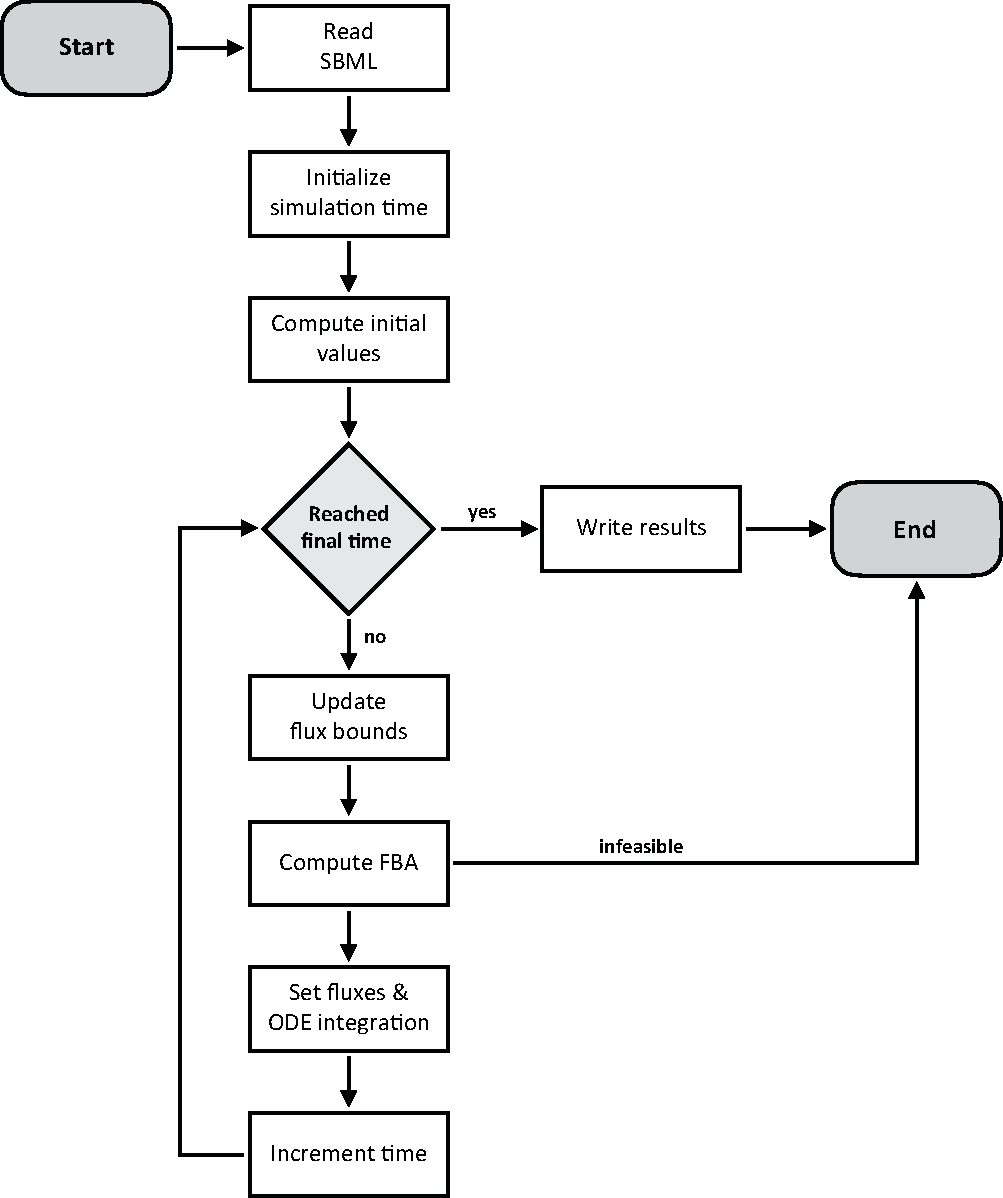
\includegraphics[width=1.0\linewidth]{figures/Fig1_simulation_algorithm.pdf}}
	\caption{Overview of the implemented SOA algorithm for DFBA. After initialization of the model, the FBA and kinetic simulations are run in an iterative manner until the simulation end point. In every step, FBA is used to compute the reaction rates of the FBA network. Subsequently, based on the computed FBA rates, the values of the species are updated dynamically. In the SOA approach, FBA fluxes are assumed to be constant within a time step. For a detailed description see the methods section.}\label{fig:sim}
\end{figure}

The first step is the initialization of the model. All of the species and parameters in the model are initialized, where each variable's initial value is computed. After the initialization step, the FBA submodel is executed. During the FBA step, reaction fluxes are computed using the initial flux bound values where the flux bounds for the reactions come from the top-level using SBML comp \emph{replacements}. In SBML, replacements of parameters and species indicate the top-level entities are the same entity as the one being replaced. Once the fluxes are computed, they are assigned to parameters using assignment rules on the top-level. These parameters are assigned reaction rates computed as functions of the fluxes.

After computing reaction fluxes, the update step is performed concurrently with the dynamic step by computing the time-evolution of every species in the UPDATE and KINETIC submodels. Species that affect any flux bound in the FBA submodel are updated in the top-level. The new bounds are used in the FBA submodel for the next time step. Simulation time is incremented at the end. If the time limit is reached, then simulation is complete. Otherwise, all of the steps are repeated. 

The SOA simulation algorithm has been implemented in \texttt{iBioSim} and \texttt{sbmlutils}. The \texttt{iBioSim} tool uses the structure of~\citep{watanabe2014} for simulation. The \texttt{sbmlutils} tool uses \emph{roadrunner}~\citep{roadrunner} for the kinetic simulation and \emph{cobrapy}~\citep{COBRAPY} to solve the FBA problem. Both \texttt{iBioSim} and \texttt{sbmlutils} take an SBML file that describes a DFBA model and a SED-ML file that describes the simulation experiment. In the proposed approach, SED-ML is mainly used to indicate which simulation algorithm to use, the time points in which tools should print out the values of the variables, the initial time and the time limit. The SED-ML files provide a minimal simulation experiment to check reproducibility between implementations. The value of each time increment for SOA is defined as a parameter with id $dt$ in the SBML model, which can be overwritten by the SED-ML file for the actual simulation.
Ontology terms for the description of DFBA simulation algorithms have been introduced in the Kinetic Simulation Algorithm Ontology (KISAO)~\citep{kisao} and are used in the SED-ML descriptions, i.e., \texttt{KISAO:0000500} (SOA-DFBA).



\subsection{Reproducibility between tools}
\label{met:reproducibility}
In order to test interoperability based on the proposed scheme, models were built in both the \texttt{iBioSim} and the \texttt{sbmlutils} tools. Models built in \texttt{iBioSim} were then imported into \texttt{sbmlutils} and vice-versa to check whether models could be interpreted by both tools consistently. This was done in an iterative manner and resulting issues were solved by clarifying the encoding scheme, e.g., by adding additional rules which resolved ambiguities.

Reproducibility of DFBA models is challenging because there may exist several possible outcomes that satisfy the objective function and constraints of the FBA models. Depending on how a solver and implementation selects one of the multiple optima different trajectories can result from the DFBA simulation. The issue of multiple optima was solved by guaranteeing uniqueness of the solution in every time step based on \emph{Flux Variability Analysis} (FVA) \citep{FVA}. FVA gives the possible minimal and maximal fluxes for each reaction in each step of the simulation. If all minimal fluxes are equal to all maximal fluxes for a time point a solution is unique in the time point. If all time points are unique the solution is unique. As a practical note: If the solution is not unique, the addition of additional constraints to the FBA problem allows to make the solution unique.

Reproducibility of the model simulations was tested by comparing the numerical SOA results between the two tools for models with unique solutions (see Supplementary Material~\nameref{sup:reproducibility}). Results were assumed as numerical identical if the absolute difference for every time point $t_k$ for all dynamical FBA species in the model $c_k$ was smaller than the tolerance $\epsilon = 1\mathrm{E}{-5}$, i.e.,
$$
abs(c_{i}(t_k)_{sbmlutils}-c_{i}(t_k)_{ibiosim}) \leq \epsilon \; \forall c_{i}, t_{k}
$$

In SOA-DFBA it is important that the time steps $dt$ are small enough so that the solution converges against the correct solution, and solutions vary if selected step sizes are too large (e.g. changing the step size in the \texttt{toy\_wholecell} model from 1.0 to 0.1 resulted in differences in steady state concentrations of up to 10\%). Consequently, different step sizes were tested for the models and step size of the simulations were selected, so that smaller step sizes did not change the simulation results.
\end{methods}

%%%%%%%%%%%%%%%%%%%%%%%%%%%%%%%%%%%%%%%%%%%%
% Results
%%%%%%%%%%%%%%%%%%%%%%%%%%%%%%%%%%%%%%%%%%%%
\section{Results}
The major result of this work is the creation of the first schema for encoding DFBA in SBML, demonstrating multi-framework computational models to be exchanged and reproduced between tools. In the following the schema and its application to multiple DFBA models is presented.

% --- Schema --- %
\subsection{Schema for dynamic flux balance analysis}
This paper proposes for the first time a schema to encode hybrid models, such as DFBA models, in SBML. The developed schema consisting of rules, guidelines, and additional information is available as Supplementary Material~\nameref{sup:guidelines}. The latest version of the document is available from \href{https://github.com/matthiaskoenig/dfba/}{https://github.com/matthiaskoenig/dfba/}. Proposals, errata, and updates to the schema are managed via the respective issue tracker and releases.

In this section we provide a high-level overview over the underlying concepts used in the schema, followed by application of the schema to encode DFBA models.

The DFBA model is constructed hierarchically using the SBML comp package, separating the hybrid model in different building blocks based on the respective functionality and modeling frameworks (Figure~\ref{fig:schema}). The top-level model is hereby composed of four submodels: (i) a kinetic submodel that computes flux bounds based on the dynamic metabolite availability and ensures that the FBA problem is constrained by the available metabolite resources (BOUNDS submodel); (ii) a FBA submodel that encodes metabolism as a FBA problem (FBA submodel); and (iii) a kinetic submodel that updates the amounts and concentrations of the dynamic metabolites changed via the FBA submodel via consumption or production (UPDATE submodel); (iv) an optional kinetic submodel that represents a dynamic part with all kinetics other than the metabolic pathway, such as DNA transcription, DNA translation, and protein degradation, among others (KINETIC submodel). Alternatively, arbitrary kinetics can be part of the top model.

%% Figure DFBA schema %%
\begin{figure}[!t]
\centerline{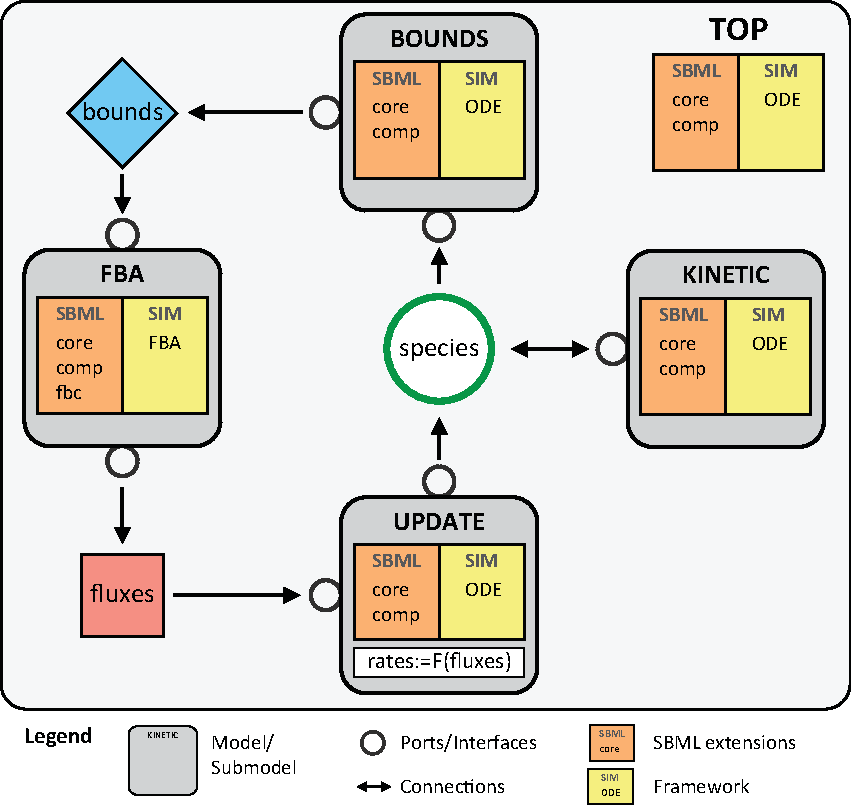
\includegraphics[width=\linewidth]{figures/Fig2_dfba_schema.pdf}}
	\caption{Overview of schema for encoding DFBA models in SBML. The hierarchical SBML model is composed of a top-level model with four submodels: FBA, BOUNDS, UPDATE, and KINETIC. The individual submodels are connected via ports. The respective SBML packages used are listed in the models, as well as the simulation framework used. The BOUNDS submodel calculates the upper and lower flux bounds based on metabolite availability. The FBA submodel computes the reaction fluxes of the metabolic fbc model using the bounds as constraints. The UPDATE submodel calculates the dynamic update of the dynamic metabolites affected by the FBA model. The rates of change are herby functions of the FBA fluxes. The KINETIC submodel includes all of the other processes in the model, which may affect or be affected by entities in metabolism. The top-level model ties together the different submodels using SBML comp replacements and replacedBy constructs.}\label{fig:schema}
\end{figure}

The top-level model ties together the three different submodels using SBML comp replacements and replacedBy constructs with the interface between the submodels defined via comp ports (which define which model components of the submodels can be connected, i.e, are exposed).
 
In order to describe the different formalisms of each submodel, the \emph{Systems Biology Ontology} (SBO) is used~\citep{SBO}. The SBO defines controlled vocabulary terms used in the systems biology field. The SBO terms are arranged in a taxonomic hierarchy using a tree structure. This allows the grouping of terms that are related to one another. The modeling formalisms of the individual submodels are described using terms on the \emph{modeling framework} branch, where FBA models are described using the \emph{flux balance framework} term, stochastic processes are described using the \emph{non-spatial discrete framework} term, and differential equations are described using the \emph{non-spatial discrete framework} term. Although the terms for stochastic processes and differential equations can be used for describing either stochastic or deterministic simulation methods, these terms were selected because they are the ones that best describes these two formalisms.

In addition to the modeling formalism other key components are annotated in the submodels via SBO terms in the schema, e.g., the upper and lower flux bounds and the exchange reactions in the FBA submodel defining which metabolites can be consumed or produced in the FBA part of the DFBA, or the dynamic species in the top model changed by the FBA submodel. By the means of these annotations the interface between the hybrid submodels can be clearly defined.

All of the interconnections between the submodels are encoded in SBML rather than using an external approach like for instance via SED-ML. The connections between model components are crucial information of the model and should be part of the model encoding. SED-ML is only used to encode which simulation to run with the model. As a consequence, this schema requires only a single hierarchical SBML model and a single SED-ML file.

%--- Toy Wholecell Example ---%
\subsection{Minimal Example (\texttt{toy\_wholecell})}
In order to illustrate the proposed schema, a simplified example of a whole-cell model was created with a model overview depicted in Figure~\ref{fig:toy_schema}. This figure shows how the different submodels connect with each other in a flat form. The model is available as COMBINE archive in Supplementary Material~\nameref{sup:toy_wholecell}, the Cytoscape visualization as Supplementary Material~\nameref{sup:toy_wholecell_cytoscape}.

This model is constructed hierarchically where a top-level model is created to instantiate different submodels (BOUNDS, UPDATE, and FBA) and make the necessary connections between them. The figure illustrates the structure of each submodel and how each submodel ties in with each other in a flat version of the model once all of the connections are established. 

In the example the FBA submodel imports species \texttt{A} and convert it via a linear chain of reactions to species \texttt{C}. The exchange reactions \texttt{EX\_A} and \texttt{EX\_C} contain the rate of consumption and production of the respective species. The TOP model contains assignment rules which assign the fluxes to the parameters \texttt{pEX\_A} and \texttt{pEX\_C}, which are used by the UPDATE model to update the dynamic species \texttt{A} and \texttt{C} via the update reactions \texttt{update\_A} and \texttt{update\_C}. The BOUNDS model calculates the bounds of all FBA exchange reactions, i.e., constraining by the availability of the dynamic species, as well as bounds changed by kinetic expressions. In the example the upper bound \texttt{ub\_R1} of reaction \texttt{R1} is changed via a rate rule. Additional kinetics are encoded in the TOP model, i.e., a kinetic conversion of \texttt{C} to \texttt{C} (these could also be in a separate KINETIC submodel).

%% Figure toy_wholecell cytoscape %%
\begin{figure*}[!t]
	\centerline{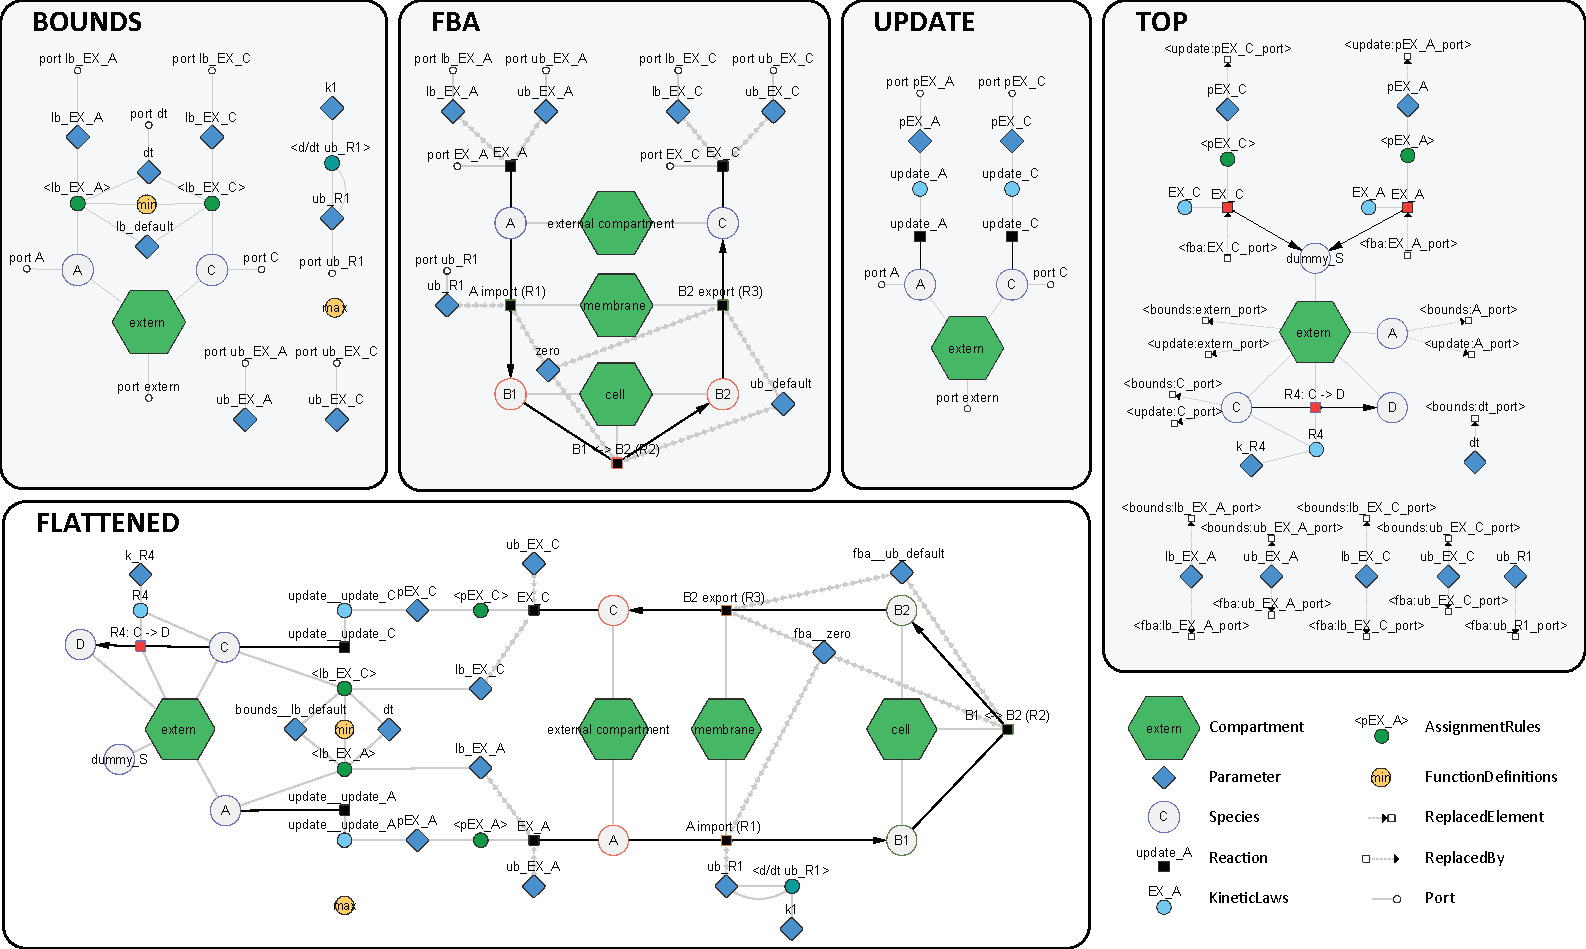
\includegraphics[width=\linewidth]{figures/Fig3_toy_wholecell_schema.pdf}}
	\caption{Detailed schema of the minimal example model (\texttt{toy\_wholecell}). The figure shows the components in the BOUNDS, FBA and UPDATE submodels. Links between submodel components are based on ports which are connected elements via TOP model replacements (replacedElements and replacedBy). The flattened SBML comp model (FLATTENED) shows the resolved connections between the different submodels after these replacements have been performed. The flattened model can not be simulated because the separation of frameworks is lost in the flattening process. The network visualization are available as interactive graphs in Cytoscape as Supplementary Material~\nameref{sup:toy_wholecell_cytoscape}, which provide additional information and annotation of the components. The figure was created with cy3sbml using the SBML models \citep{CySBML}.}\label{fig:toy_schema}
\end{figure*}

In order to validate the exchangability and reproducibility of the model, simulations were performed using the simulation algorithm described in Figure~\ref{fig:sim} with results depicted in Figure~\ref{fig:toy_results}. Both implementations resulted in numerically identical results (see \ref{met:reproducibility}).
Importantly, our encoding schema allowed to reproduce the numerical results even if the step sizes were not yet small enough to have converged against the correct solution, thereby allowing to test the effects of varying step sizes in a reproducible manner.

%% Figure toy wholecell results %%
\begin{figure*}[!t]
\begin{subfigure}[t]{0.5\textwidth}	\centerline{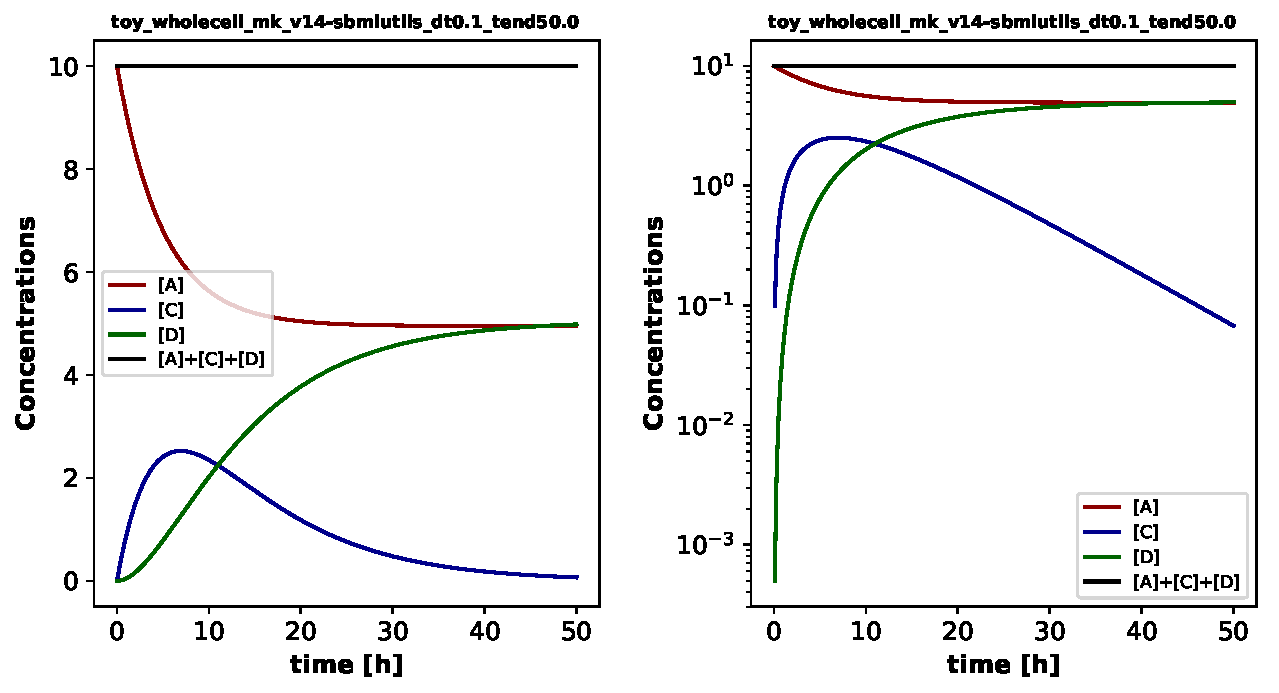
\includegraphics[width=\linewidth]{figures/Fig4_toy_wholecell_mk_v14-sbmlutils_dt0_1_tend50_0.pdf}}
	\caption{Simulation results with \texttt{sbmlutils}}\label{fig:sbmlutils_toy_results}
\end{subfigure}
~
\begin{subfigure}[t]{0.5\textwidth}	\centerline{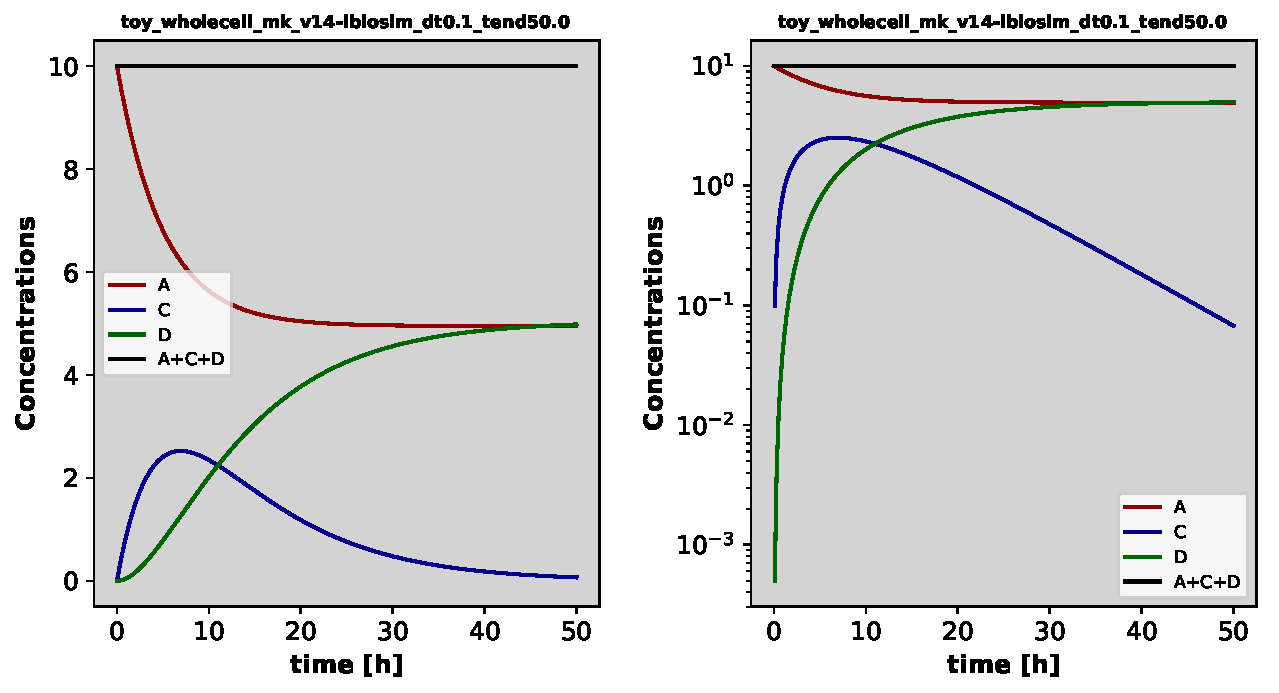
\includegraphics[width=\linewidth]{figures/Fig4_toy_wholecell_mk_v14-ibiosim_dt0_1_tend50_0.pdf}}
	\caption{Simulation results with \texttt{iBioSim}}\label{fig:biosim_toy_results}
\end{subfigure}
\caption{DFBA Simulation results for the \texttt{toy\_wholecell} model in two different tools. This demonstrates that models can be exchanged by different tools using standards and the results can be reproduced when using the same simulation algorithm. Species \texttt{A} is converted to \texttt{C} via the FBA subnetwork over time. \texttt{C} is converted to \texttt{D} via the kinetic parts in the top model. Species \texttt{A} is not consumed completely because the import of \texttt{A} in the FBA subnetwork via \texttt{R1} is shut down via a rate rule for the upper flux bound, and a steady state is reached. The model was simulated for 50[h] with a time step \texttt{dt} of 0.1[h].}
\label{fig:toy_results}
\end{figure*}

In addition to the presented minimal model, a second model of a simplified DFBA glycolysis (\texttt{toy\_atp}) is available in the supplement (COMBINE archive in Supplementary Material~\nameref{sup:toy_atp}, corresponding Cytoscape visualization in Supplementary Material~\nameref{sup:toy_atp_cytoscape}).

% --- DIAUXIC GROWTH --- %
\subsection{Diauxic growth in \emph{E. coli} (\texttt{diauxic\_growth})}
The next example is an encoding and reproduction of results from a published DFBA model of diauxic growth of \emph{E.~coli~}\citep{DFBA_ECOLI} consisting of four reactions between four metabolites, i.e., glucose ($Glcxt$), oxygen ($O_2$), acetate ($A_c$) and biomass ($X$). The model can grow either aerobically on acetate ($v1$), aerobically on glucose ($v2$ or $v3$) or anaerobically convert glucose to acetate:

\begin{align*}
v1&: 39.43 A_c + 35 O_2 \rightarrow X \\
v2&:  9.46 Glcxt + 12.92 O_2 \rightarrow X \\
v3&: 9.84 Glcxt + 12.73 O_2 \rightarrow 1.24 A_c + X \\
v4&: 19.23 Glcxt \rightarrow 12.12 A_c + X \\
\end{align*}
The kinetic part of the model is described by the following differential equations:
\begin{align*}
\frac{d Glcxt}{dt} &= A^{Glcxt} \nu X \\
\frac{d A_c}{dt} &= A^{A_c} \nu X \\
\frac{d O_2}{dt} &= A^{O_2} \nu X + k_L a(0.21 - O_2) \\
\frac{d X}{dt} &= (v1 + v2 + v3 + v4) X\\
\end{align*}
where $A^{Glcxt}$, $A^{A_c}$, $A^{O_2}$ are the respective rows of each variable in the stoichiometry matrix and $k_L a$ is the mass transfer coefficient of oxygen. For a detailed description see~\citep{DFBA_ECOLI}. 

The model is available in Supplementary Material~\nameref{sup:diauxic_growth}, the Cytoscape visualization in Supplementary Material~\nameref{sup:diauxic_growth_cytoscape}.

The results in Figure~\ref{diauxic_example} depict an exponential growth phase using glucose aerobically until running out of glucose, which at this point the cell grows linearly due to oxygen. When both oxygen and glucose run out, the cell growth stagnates. Experimental data from~\citep{DFBA} is plotted alongside the simulation results. The model is able to capture the behavior observed in the experimental data. The results are equivalent to the models in~\citep{DFBA_ECOLI}.

%% Figure diauxic growth results %%
\begin{figure*}[!t]
%\begin{subfigure}[t]{0.5\textwidth}	\centerline{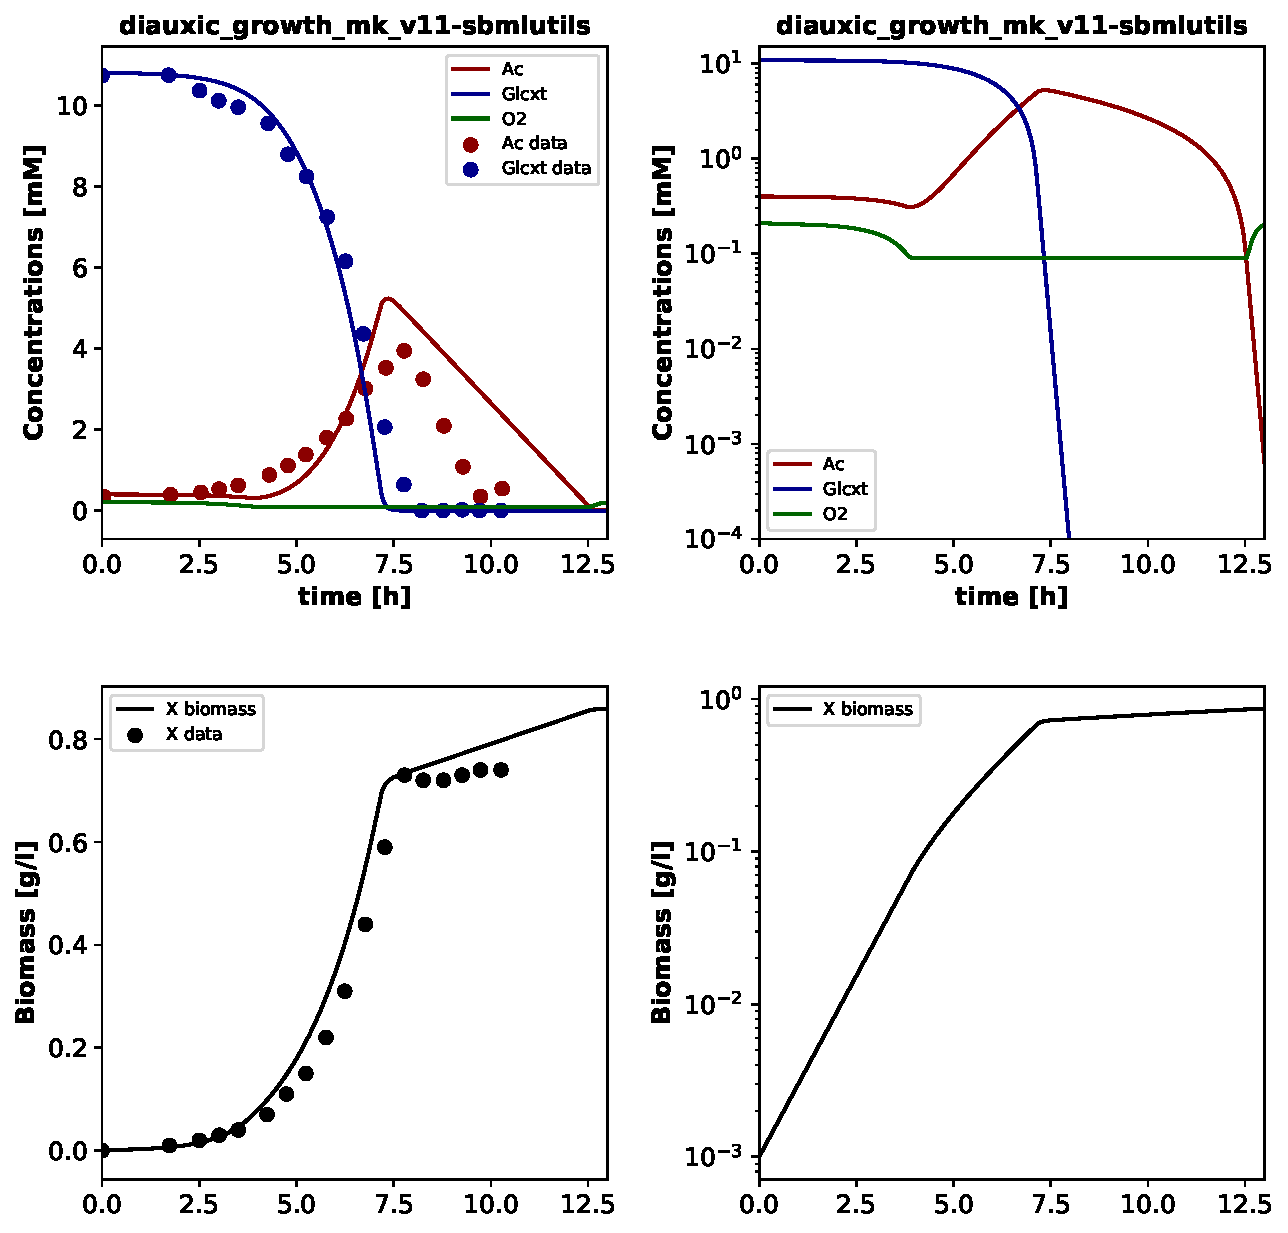
\includegraphics[width=\linewidth]{figures/Fig5_diauxic_growth_mk_v11-sbmlutils.pdf}}
\begin{subfigure}[t]{0.5\textwidth}	\centerline{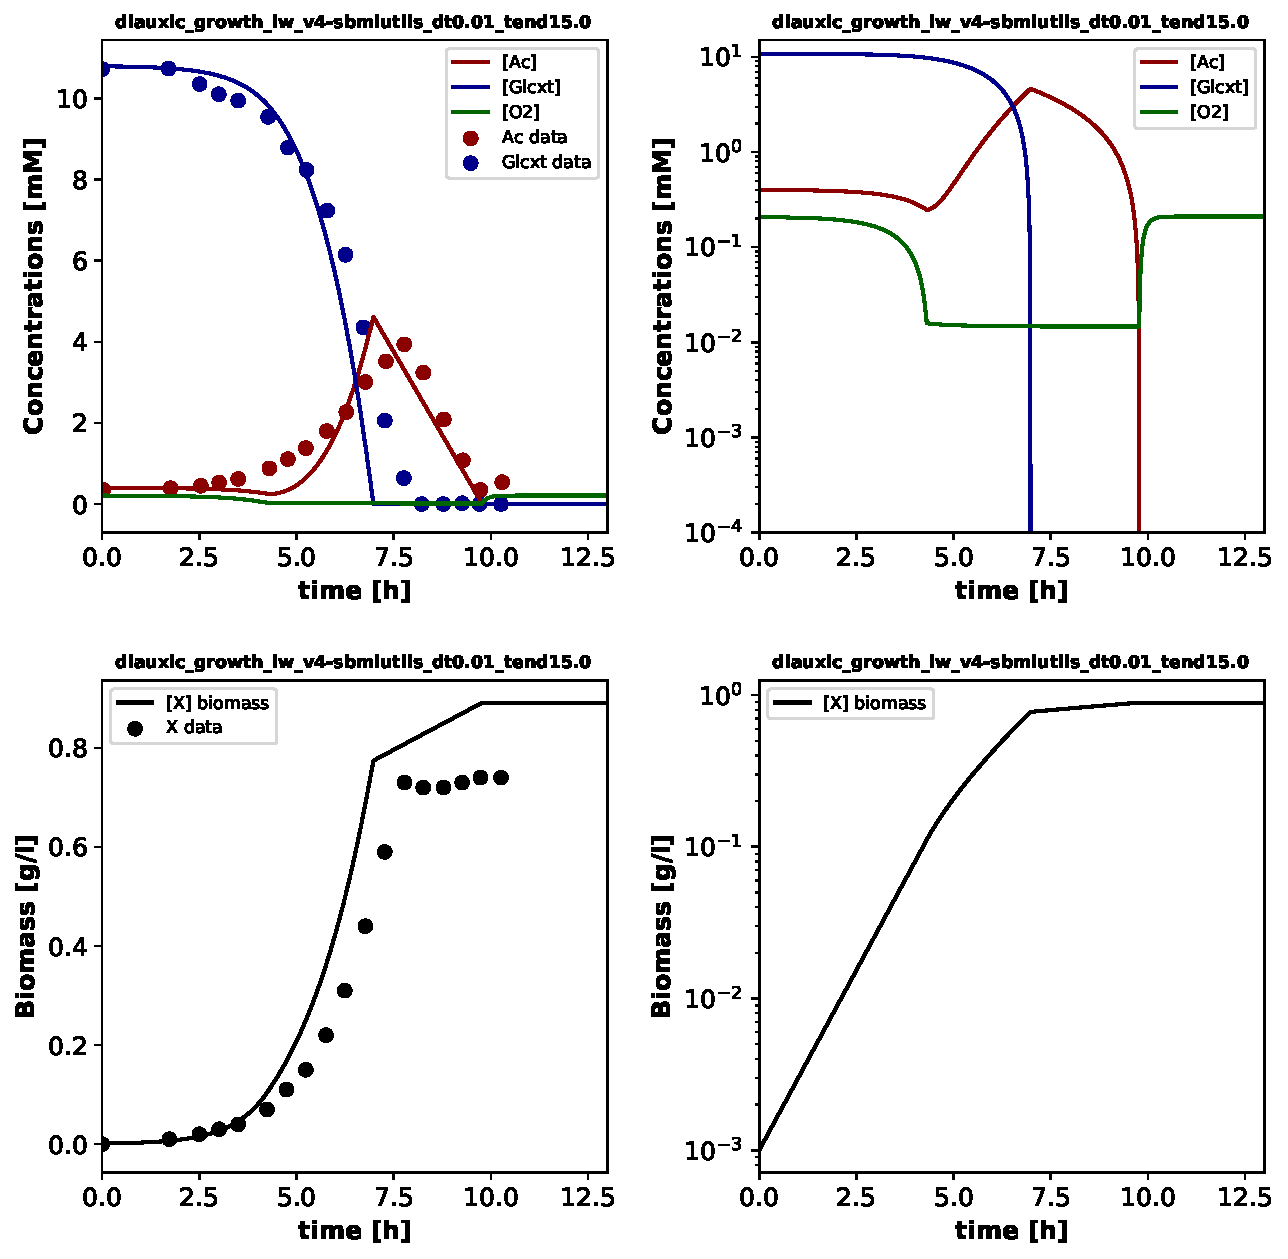
\includegraphics[width=\linewidth]{figures/Fig5_diauxic_growth_lw_v4-sbmlutils_dt0_01_tend15_0.pdf}}

	\caption{This is the simulation results for the diauxic growth of \emph{E. Coli} in \texttt{sbmlutils}.}\label{diauxic_sbmlutils}
    \end{subfigure}
    ~
    \begin{subfigure}[t]{0.5\textwidth}	\centerline{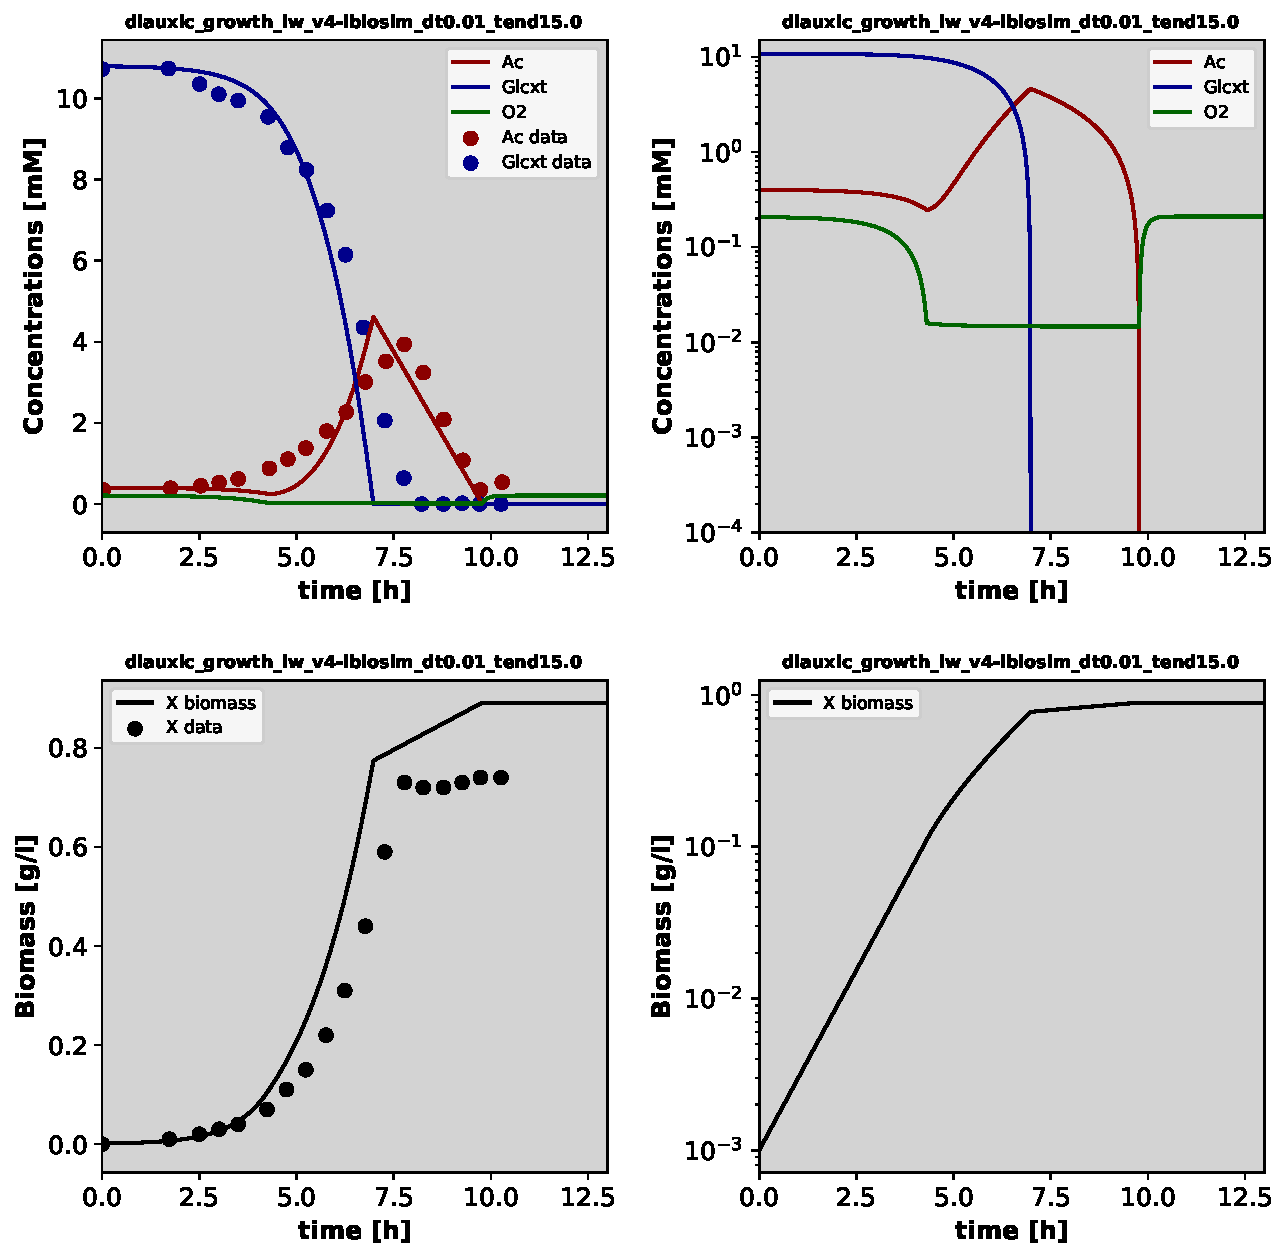
\includegraphics[width=\linewidth]{figures/Fig5_diauxic_growth_lw_v4-ibiosim_dt0_01_tend15_0.pdf}}
	\caption{This is the simulation results for the diauxic growth of \emph{E. Coli} simulated in \texttt{iBioSim}. }\label{diauxic_ibiosim}
    \end{subfigure}
    \caption{This plot shows the results for the model representing diauxic growth in \emph{E. coli}. The model is able to reproduce the general behavior captured from experiment data. There is an exponential cell growth while glucose is present in the model, but when the cell runs out of glucose, growth slows down and is affected mostly by oxygen. However, when the cell runs out of glucose and oxygen, growth diminishes significantly. The model was simulated for 15[h] with a time step \texttt{dt} of 0.01[h].}\label{diauxic_example}
\end{figure*}

We hereby showed that our schema is able to encode published DFBA models, resulting in a reproducible and exchangeable model representation between tools.

% --- E.COLI CORE --- %
\subsection{\emph{E. coli} core (\texttt{ecoli})}
To demonstrate the feasibility of the proposed schema and method for real-world examples of DFBAs, a larger metabolic network for the core metabolism of \emph{E. coli}~\citep{ecoli_core} was encoded in the proposed schema and simulated as shown in Figure~\ref{fig:ecoli}. The model is available as COMBINE archive in Supplementary Material~\nameref{sup:ecoli}. The FBA submodel was downloaded from BiGG \citep{bigg} (core metabolism of Escherichia coli str. K-12 substr. MG1655) and transformed to an DFBA model in an automatic fashion using \texttt{sbmlutils}. BiGG models encode the exchangeable species via annotated exchange reactions which allows and automatic inference of the dynamic species. Only additional information required to run a DFBA simulations are initial concentrations for the species. The automatic encoding of larger scale examples demonstrates the scalability of the proposed encoding approach. 

\begin{figure}[!t]
	\centerline{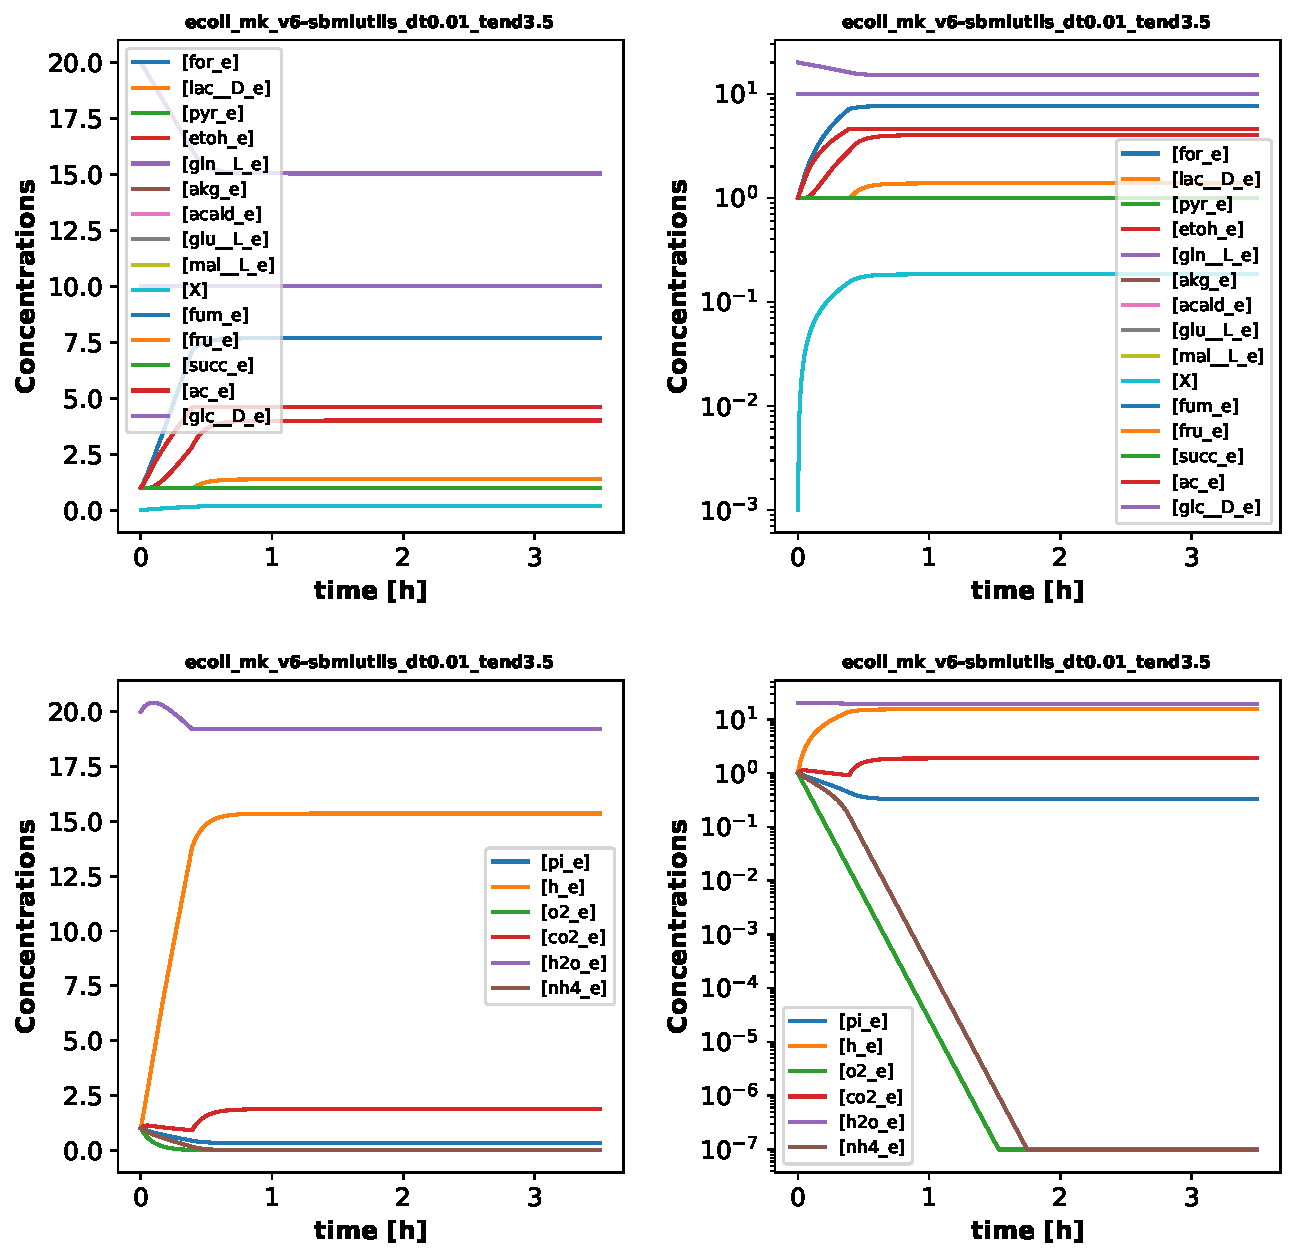
\includegraphics[width=\linewidth]{figures/Fig6_ecoli_mk_v6-sbmlutils_dt0_01_tend3_5.pdf}}
	\caption{DFBA simulation results for core metabolism of \emph{E. coli} with sbmlutils. The proposed approach can be used in larger models, such as the \emph{E. coli} model described in the paper. The model is growing aerobically on glucose in the initial phase and reaches a steady state after oxygen is consumed. The model was simulated for 3.5[h] with a time step \texttt{dt} of 0.01[h].}\label{fig:ecoli}
\end{figure}

While \texttt{sbmlutils} is able to find a solution for the model, \texttt{iBioSim} cannot as it runs into an unfeasible solution in the middle of simulation. This captures the well-known problem of DFBA with multiple solutions. The FBA problem is not constrained enough to result in a unique solution and  depending on which solution the simulator picks, different solutions and thereby trajectories arise. Despite the existence of multiple solutions, tools and LP solver typically pick solutions deterministically. Hence, single tools can reproduce their own results, but results are irreproducible between different implementation. Without the use of standards, this could never be demonstrated because variations in results could be due to discrepancies in the model, and not in the tool.

%%%%%%%%%%%%%%%%%%%%%%%%%%%%%%%%%%%%%%%%%%%%
% DISCUSSION
%%%%%%%%%%%%%%%%%%%%%%%%%%%%%%%%%%%%%%%%%%%%
\section{Discussion}

Modularity of models, the ability to encode multi-framework models, and reproducibility of models is indispensable for encoding more complex models in computational biology. In this work we presented such an approach, which allows a clear separation of the different modeling frameworks via comp submodels and defining the interfaces between the submodels.
To our knowledge, this paper proposes and implements for the first time an exchangeable and reproducible multi-framework scheme. This scheme for encoding DFBA models in a standard way has been implemented in two different tools, demonstrating the exchangeability and reproducibility of our approach on various examples models like diauxic growth in \emph{E.coli}. \texttt{iBioSim} and \texttt{sbmlUtils} are freely available for download and offer the necessary infrastructure for anyone to develop DFBA models using the proposed scheme.

Currently, the proposed approach supports the modeling of DFBA models based on the SOA simulation algorithm. Hence, our approach only covers a subset of DFBA algorithms and possible frameworks which could be coupled.

Most DFBA models are stiff and small time steps are required for stability, making the SOA approach computationally expensive. Another disadvantage of the SOA approach is that it requires a sufficiently small fixed time step to give accurate results. Future directions include the exploration of adaptive time steps for executing the DFBA with SOA, alternative DFBA methods, such as DOA or DA, and extending our scheme to encode such models.

Our current is limited to the coupling of ODE and FBA frameworks. Different types of hybrid model, such as a mixture of differential equations, stochastic processes, and boolean models still need further study. The proposed approach of decoupling frameworks via hierarchical model composition could work similarly for other modeling frameworks like boolean models.

So far, only small to medium-size DFBA models have been encoded in our proposed approach. For future work, we will encode genome-scale metabolic models. This would allow us to assess the scalability and performance of the proposed approach.

%%%%%%%%%%%%%%%%%%%%%%%%%%%%%%%%%%%%%%%%%%%%
% ACKNOWLEDGEMENTS
%%%%%%%%%%%%%%%%%%%%%%%%%%%%%%%%%%%%%%%%%%%%
\section*{Acknowledgements}
The authors would like to thank Frank Bergmann and Ilya Kiselev for participating in the discussions for this work.

\section*{Funding}
LW and CM are supported by the National Science Foundation under Grants CCF-1218095 and CCF-1748200. Any opinions, findings, and conclusions or recommendations expressed in this material are those of the author(s) and do not necessarily reflect the views of the National Science Foundation. MK is supported by the Federal Ministry of Education and Research (BMBF, Germany) within the research network Systems Medicine of the Liver (LiSyM) (grant number 031L0054). 

%%%%%%%%%%%%%%%%%%%%%%%%%%%%%%%%%%%%%%%%%%%%
% SUPPLEMENTARY
%%%%%%%%%%%%%%%%%%%%%%%%%%%%%%%%%%%%%%%%%%%%
\section*{Supplementary Material}
\paragraph*{S1} \label{sup:guidelines} Schema for encoding DFBA in SBML
\paragraph*{S2} \label{sup:reproducibility} Reproducibility results between sbmlutils and iBioSim
\paragraph*{S3} \label{sup:toy_wholecell} \texttt{toy\_wholecell} Minimal DFBA model COMBINE archive
\paragraph*{S4} \label{sup:toy_wholecell_cytoscape} \texttt{toy\_wholecell} Minimal DFBA model Cytoscape session file
\paragraph*{S5} \label{sup:toy_atp} \texttt{toy\_atp} Minimal glycolysis DFBA model COMBINE archive
\paragraph*{S6} \label{sup:toy_atp_cytoscape} \texttt{toy\_atp} Minimal glycolysis DFBA model Cytoscape session file
\paragraph*{S7} \label{sup:diauxic_growth} \texttt{diauxic} Diauxic DFBA model COMBINE archive
\paragraph*{S8} \label{sup:diauxic_growth_cytoscape} \texttt{diauxic} Diauxic DFBA model Cytoscape session file
\paragraph*{S9} \label{sup:ecoli} \texttt{ecoli} E.coli core DFBA model COMBINE archive

\bibliographystyle{natbib}
\bibliography{ref}

\end{document}
